\chapter{Diagrams of Neural Networks}
\label{app:NN_Architecture}
%%%%%%%%%%%%%%%%%%%%%%%%%%%%%%%%%%%%%%%%%%%%%%%%%%%%%%%%%%%%%%%
\begin{figure}[h!]
    \centering
    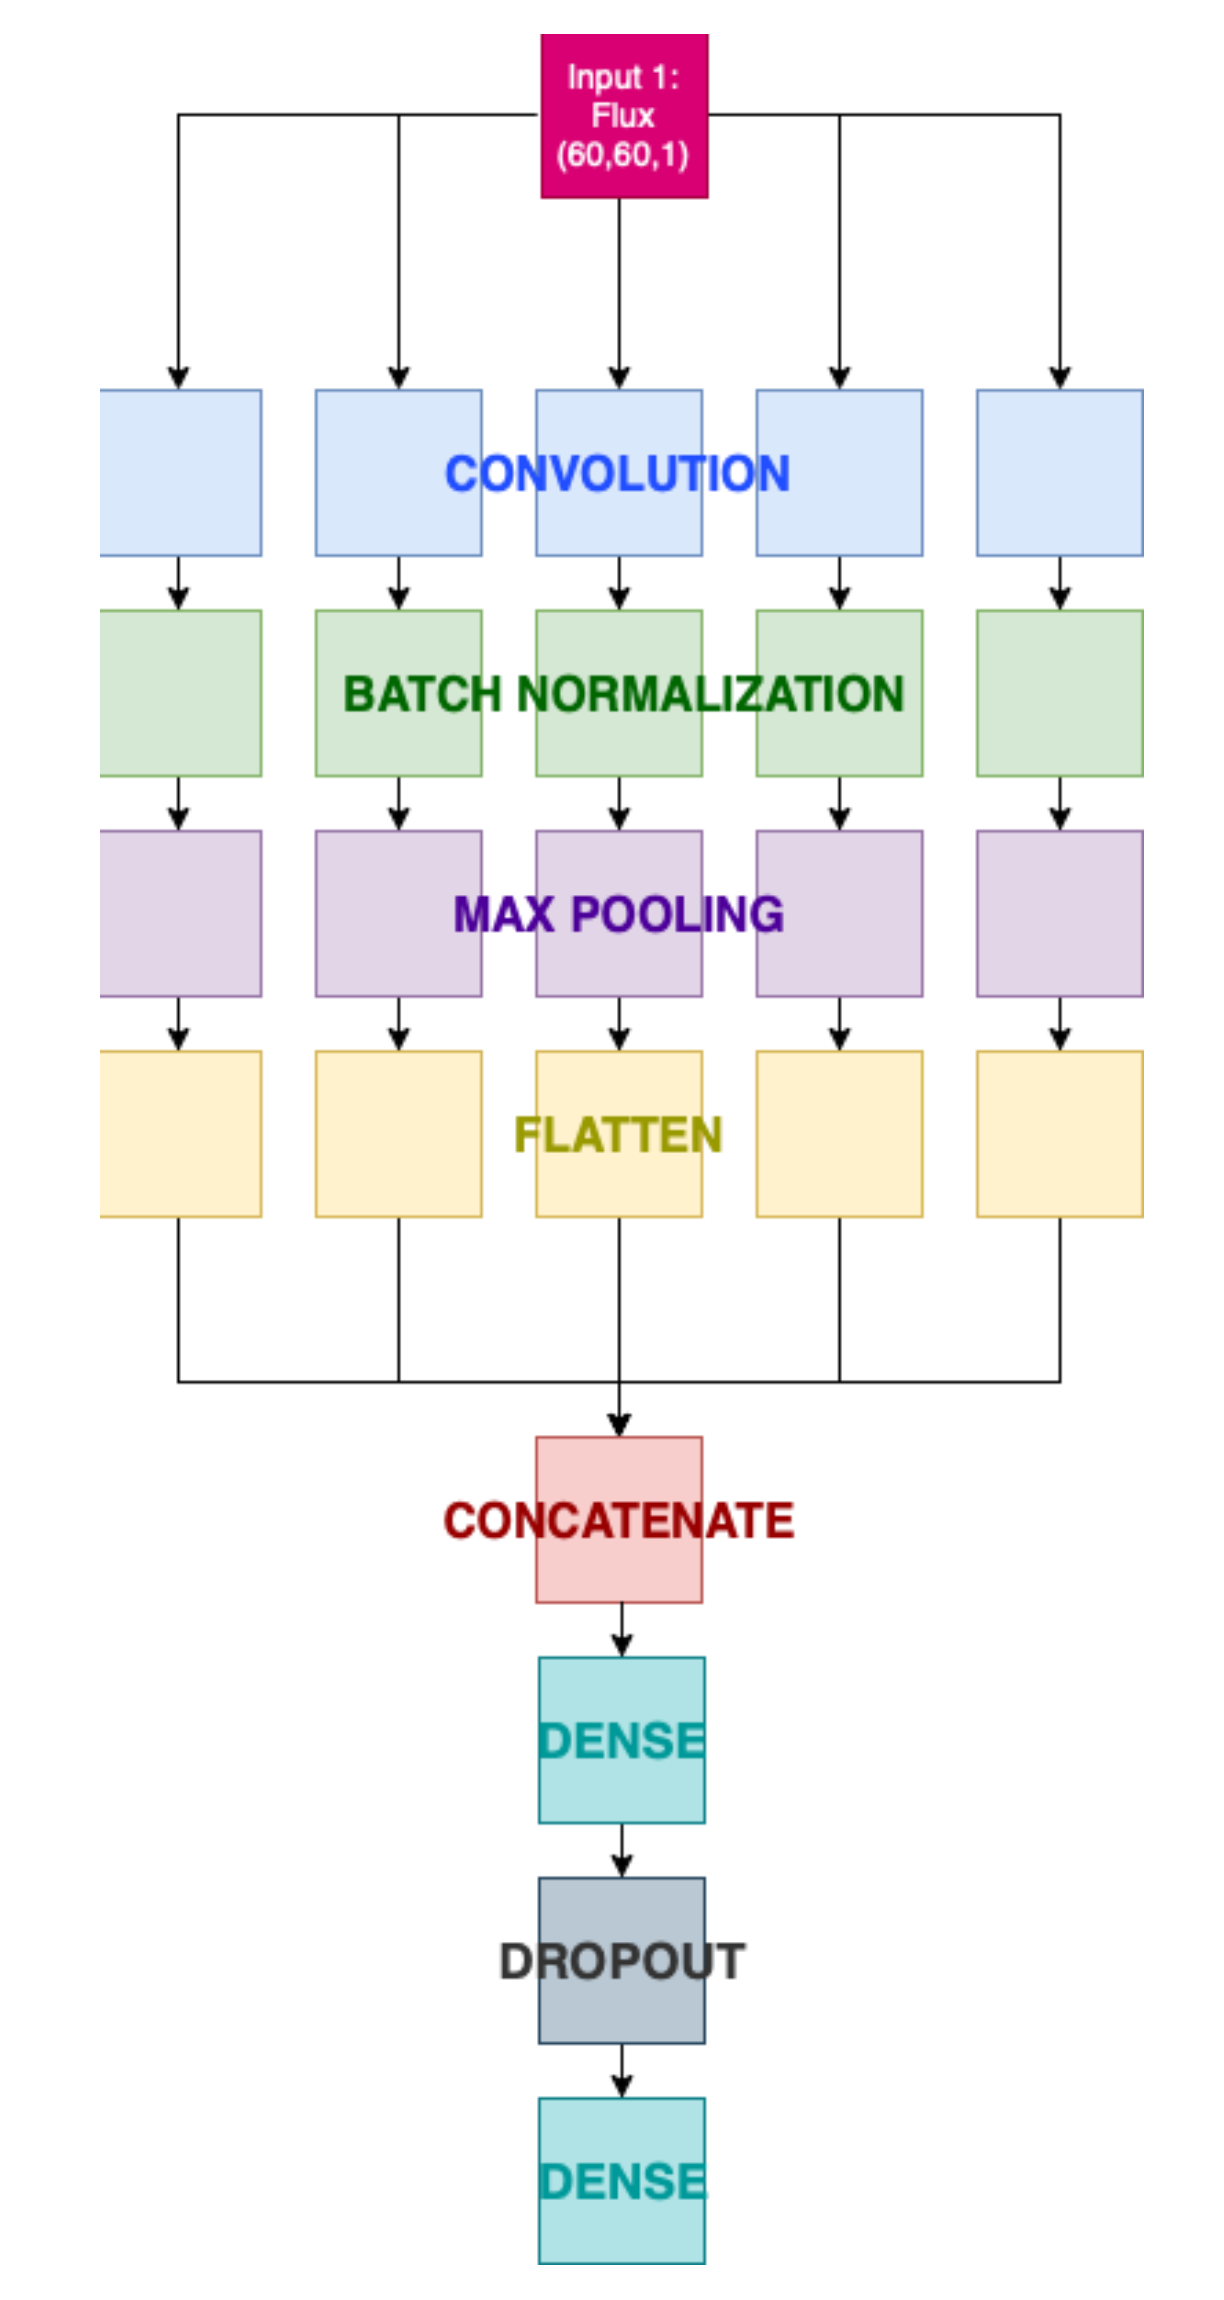
\includegraphics[height=.4\pdfpageheight]{figures/EddieCNN.png}
    \caption{CNN architecture. Figure from \textcite{Sepeku2022}.}
    \label{fig:cnn_architecture}
\end{figure}

\clearpage
\begin{figure}
    \centering
    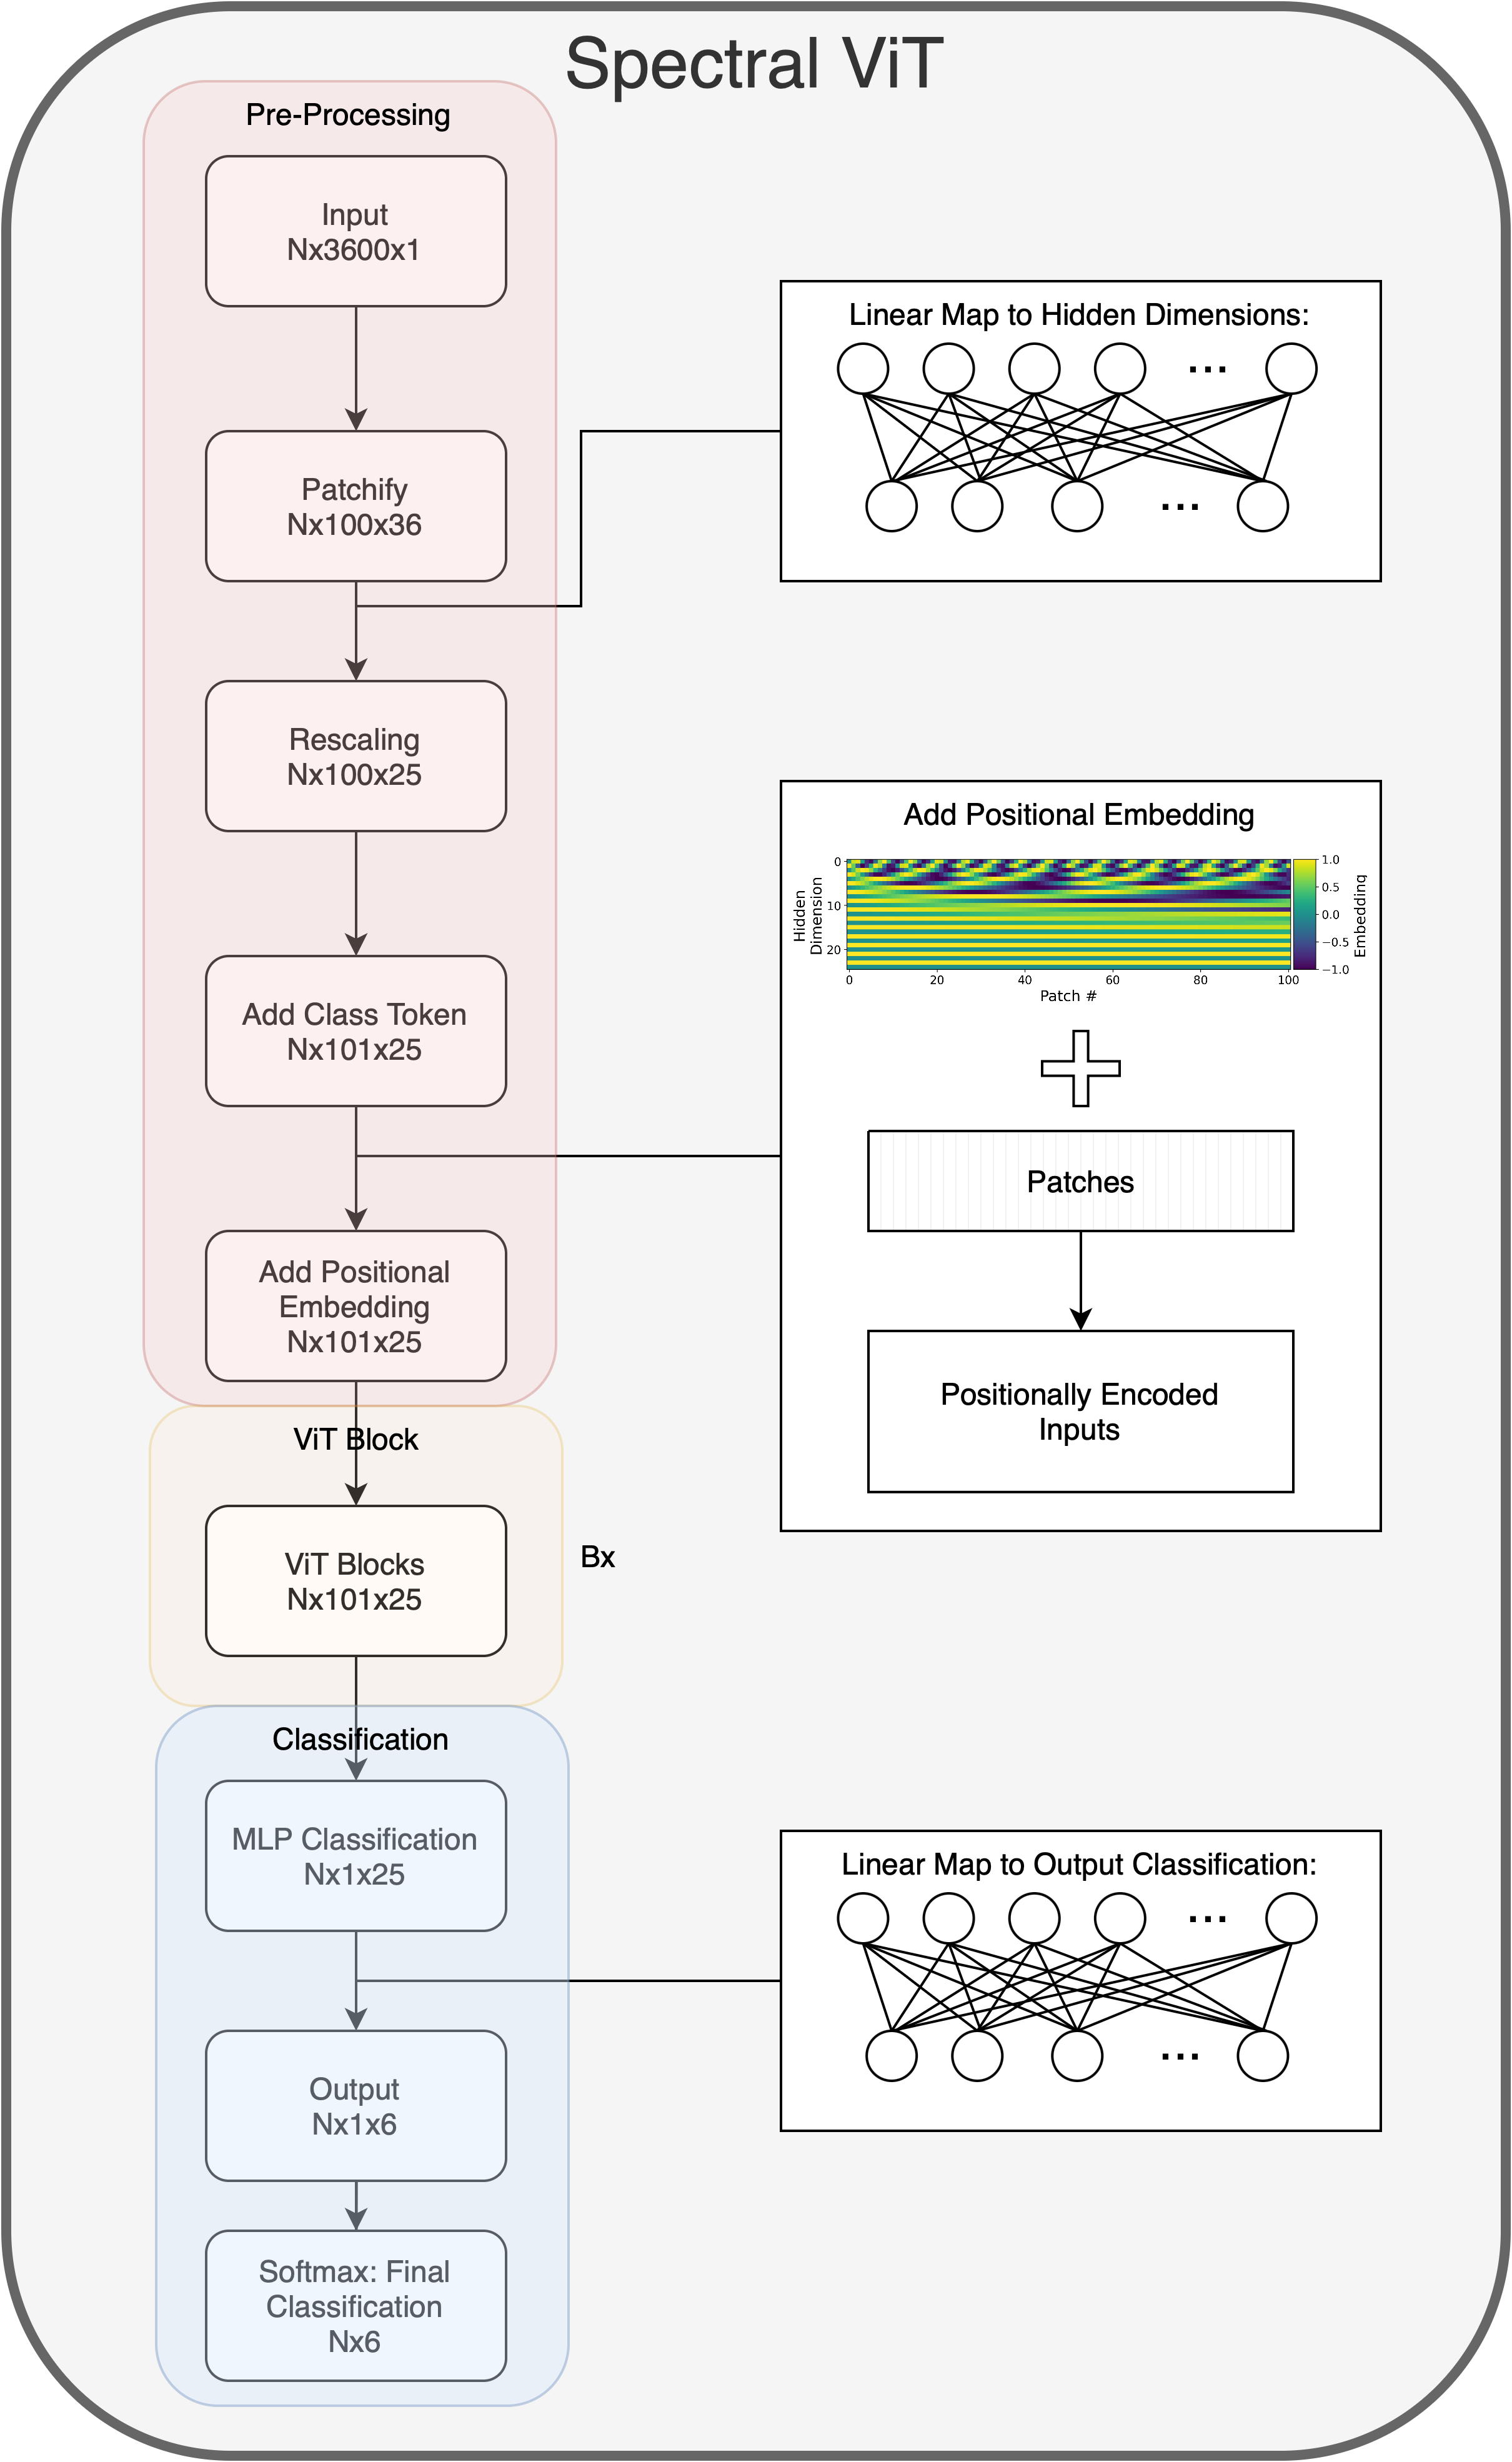
\includegraphics[height=.7\pdfpageheight]{figures/TransformerDiagrams/SpectralViT.png}
    \caption{Spectral ViT Architecture}
    \label{fig:SpectralViTDiag}
\end{figure}

\begin{figure}
    \centering
    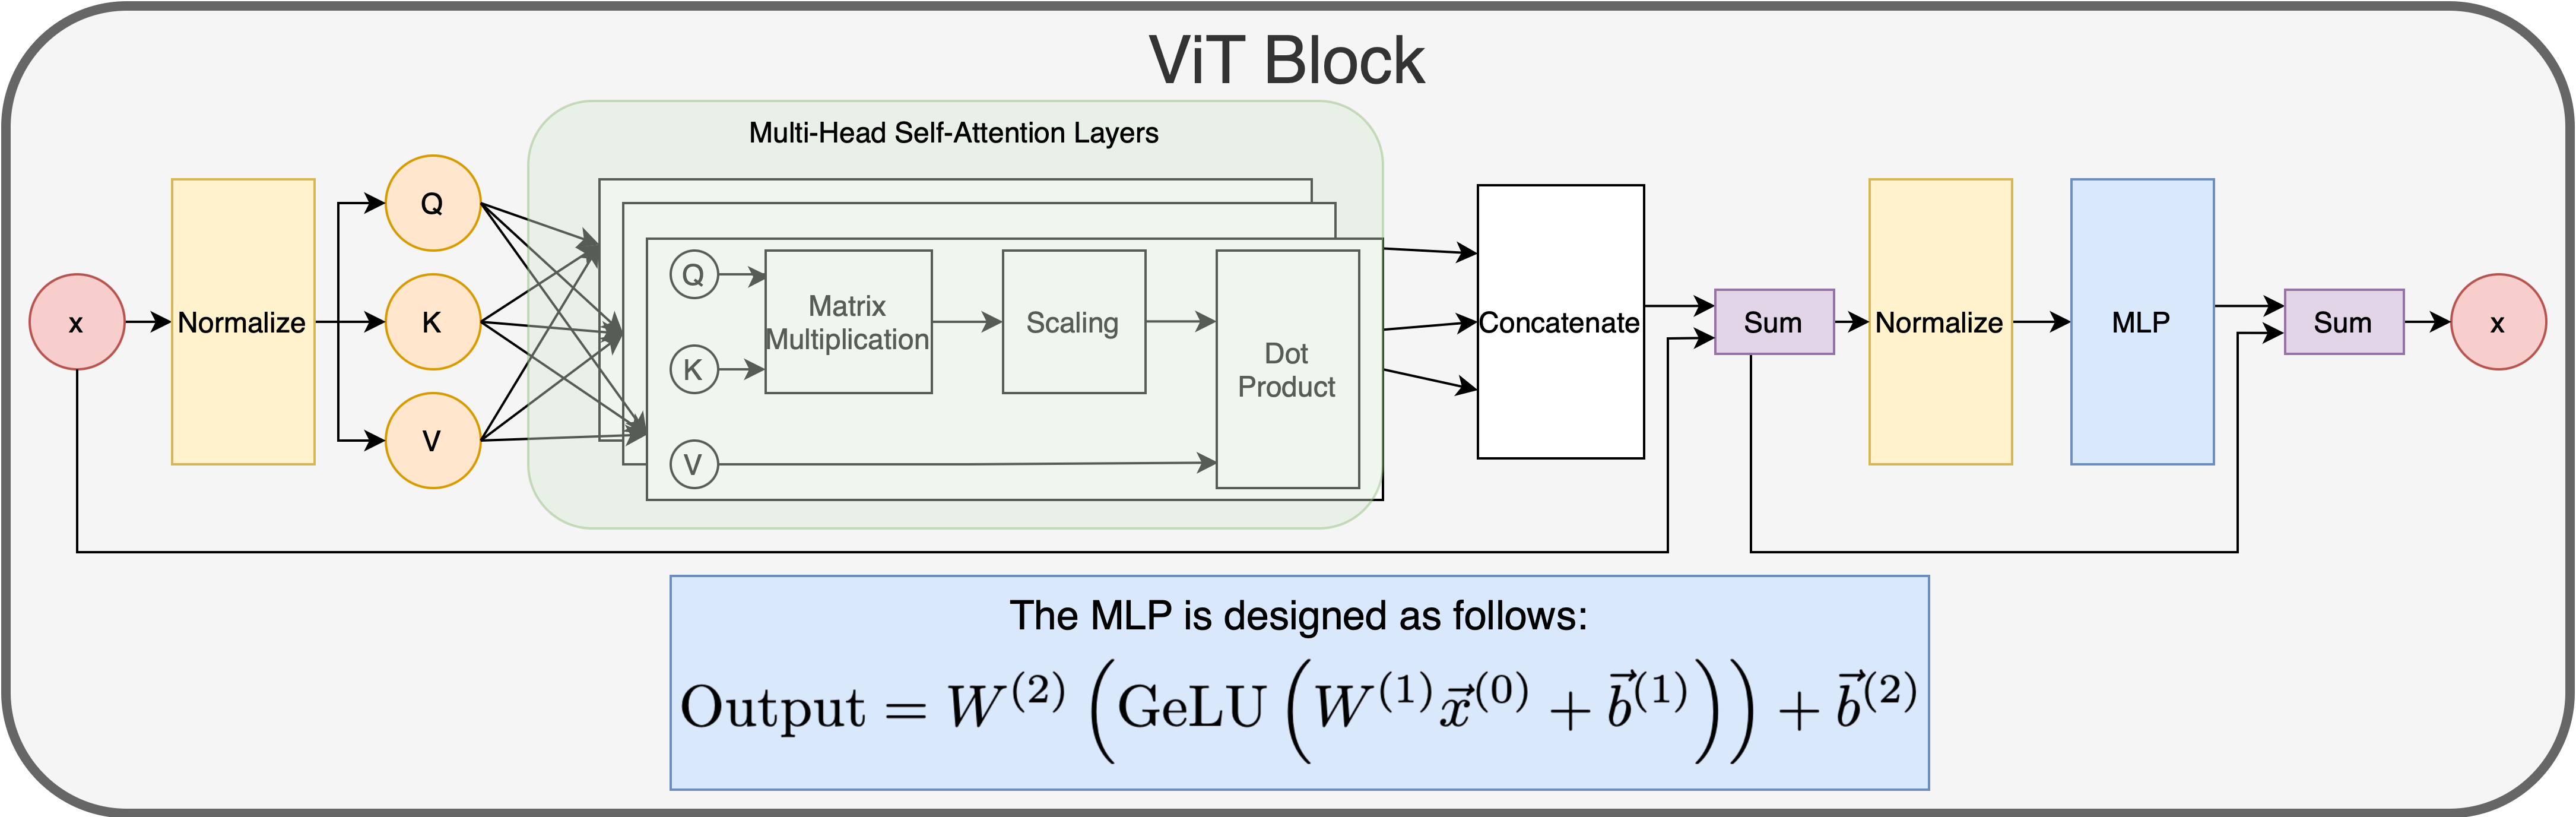
\includegraphics[width=\textwidth]{figures/TransformerDiagrams/Attention.png}
    \caption[Spectral ViT Block]{The ViT Block Subarchitecture includes the mutli-head 
    self attention layers, a normalization layer, and an MLP.}
    \label{fig:SpectralViTBlock}
\end{figure}
